\chapter{}\label{chap:intro}


%\usepackage{graphicx, epsfig}
%\usepackage{epstopdf}
%\usepackage{color}
%\usepackage{mathrsfs}
%\usepackage{amsmath}


%\input epsf
%\tighten


 %%%%%%%%%%%%%%%%%%%%%%%%%%%%%%%%%%%%%%%%%%%%%%%%%%%%%%%



\section{Introduction}
Lorem ipsum dolor sit amet, consectetur adipiscing elit, sed do eiusmod tempor incididunt ut labore et dolore magna aliqua. Convallis aenean et tortor at risus viverra adipiscing at. Rutrum tellus pellentesque eu tincidunt tortor aliquam nulla facilisi cras. Luctus accumsan tortor posuere ac ut consequat semper viverra nam. Lectus nulla at volutpat diam ut venenatis tellus in metus. Nibh mauris cursus mattis molestie a iaculis at. Egestas quis ipsum suspendisse ultrices gravida dictum fusce. Lacinia at quis risus sed. Ut venenatis tellus in metus vulputate. Tortor at risus viverra adipiscing. Aliquam vestibulum morbi blandit cursus risus at ultrices. Neque volutpat ac tincidunt vitae. In massa tempor nec feugiat.
Equations can also look like \ref{eq2}

\begin{equation}
\label{eq2}
V(r) = \left\{
\begin{array}{ll}
+\infty & \quad r < 2a \\
0 & \quad r > 2a
\end{array}
\right.
\end{equation}

\section{}
Lorem ipsum dolor sit amet, consectetur adipiscing elit, sed do eiusmod tempor incididunt ut labore et dolore magna aliqua. Convallis aenean et tortor at risus viverra adipiscing at. Rutrum tellus pellentesque eu tincidunt tortor aliquam nulla facilisi cras. Luctus accumsan tortor posuere ac ut consequat semper viverra nam. Lectus nulla at volutpat diam ut venenatis tellus in metus. Nibh mauris cursus mattis molestie a iaculis at. Egestas quis ipsum suspendisse ultrices gravida dictum fusce. Lacinia at quis risus sed. Ut venenatis tellus in metus vulputate. Tortor at risus viverra adipiscing. Aliquam vestibulum morbi blandit cursus risus at ultrices. Neque volutpat ac tincidunt vitae. In massa tempor nec feugiat.

We can also add tables like Table~\ref{tabdeloc}

\begin{table}[!h]

	\begin{center}

		\begin{tabular}{|c|c|c|c|}
			\hline N & M &  $\ket{\psi_i}$ & $\mathcal{N}[\psi_i]$ \\ 
			\hline 5 & 10 & $a^\dagger_i$ & $\approx$695 \\ 
			\hline 5 & 10 &  $a^\dagger_3a^\dagger_4$ & 3181 \\ 
			\hline 5 & 16 &  $a^\dagger_i$ & $\approx$1791 \\ 
			\hline 5 & 16 &  $a^\dagger_3a^\dagger_4$ & 10858 \\ 
			\hline 5 & 20 &  $a^\dagger_i$ & $\approx$2950 \\ 
			\hline 5 & 20 &  $a^\dagger_3a^\dagger_4$ & 20801 \\ 
			\hline 
		\end{tabular} 
	\end{center}
	\caption{Sample table. }\label{tabdeloc}
\end{table} 

To add multiple subfigures do as shown in Fig.(\ref{multfig}) instead of Fig.(\ref{infspring})

\begin{figure}[ht]
	\centering
	\begin{subfigure}[h]{0.45\textwidth}
		\centering
		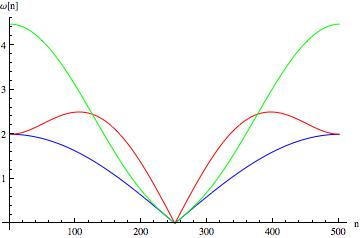
\includegraphics[height=0.7\linewidth,width=\linewidth]{chapter-2/fig/dispersion}
		\caption{subFig 1}
		
	\end{subfigure}
	\begin{subfigure}[h]{0.45\textwidth}
		\centering
		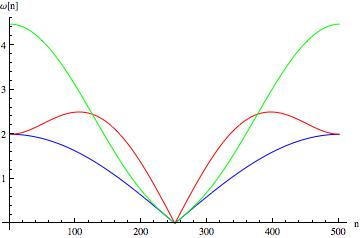
\includegraphics[height=0.7\linewidth,width=\linewidth]{chapter-2/fig/dispersion}
		\caption{subFig 2}
		
	\end{subfigure}
	\centering
	\begin{subfigure}[h]{0.45\textwidth}
		\centering
		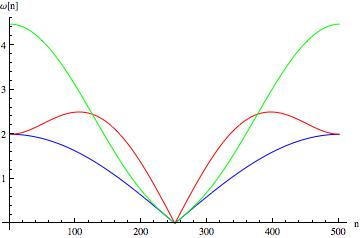
\includegraphics[height=0.7\linewidth,width=\linewidth]{chapter-2/fig/dispersion}
		\caption{subFig 2}
		
	\end{subfigure}
	\caption{All subfigures are together}
	\label{multfig}

\end{figure}
\FloatBarrier
	
You can modify the sizes and shapes of the subfigures as you wish and depending on your preference for the position of these figures with the "htb!" commands. You can use packages like \textbackslash FloatBarrier to prevent \LaTeX from pushing the figures to other pages.


%\newpage




